\section{JPEG}\label{sec:jpeg}

\subsection{JPEG-Kompression}\label{subsec:jpeg-kompression}

\begin{enumerate}[label={\bfseries Schritt \arabic*:}, wide=0pt]
    \item \textbf{Transformation Farbbilder RGB $\Rightarrow$ Luminanz / Chrominanz}

    Das Auge ist empfindlicher auf kleine Helligkeitsunterschiede als auf kleine Farbunterschiede, d.h.\ die Farbinformation kann höher komprimiert werden, ohne dass man es merkt (Irrelevanz).

    \item \textbf{Downsampling der beiden Chrominanz-Komponenten}

    \begin{itemize}
        \item 2:1 horizontal und vertikal (2h2v oder 4:2:0) \\
        $\Rightarrow$ Bildgrösse: $1/3 + (2/3) \cdot (1/4) = 1/2$
        \item 2:1 horizontal und 1:1 vertikal (2h1v oder 4:2:2) \\
        $\Rightarrow$ Bildgrösse: $1/3 + (2/3) \cdot (1/2) = 2/3$
    \end{itemize}

    \item \textbf{Pixel-Gruppierung der Farbkomponenten in 8x8 Blöcke}

    In diesem Schritt werden die horizontalen und vertikalen Korrelation ausgenutzt.
    Blöcke werden separat komprimiert, was die Schwachstelle von JPEG ist.

    \item \textbf{Diskrete Cosinustransformation (8x8 DCT)}

    Transformation in den Frequenzbereich, was die Vorbereitung für die Datenkompression ist.
    DC und 3--4 tieffrequente AC-Werte enthalten die ``Bildinformation''.

    \item \textbf{Individuelle Quantisierung einzelner Frequenzkomponenten}

    Im Prinzip werden die Frequenzkomponenten mit viel bzw.\ wenig Bildinformation fein bzw.\ grob quantisiert.

    \item \textbf{Entropiecodierung der quantisierten Frequenzkomponenten}

    Dieser Schritt verläuft verlustlos und ist eine Kombination von RLE und Huffman-Encoding.

    \item \textbf{Hinzufügen von Header und JPEG Parameter}
\end{enumerate}

\begin{definition}{Zweidimensionale DCT}
    \begin{itemize}
        \item \textbf{Forward DCT (JPEG: 8x8)} \[F_{vu} = \frac{1}{4} C_u C_v \sum_{x=0}^{7} \sum_{y=0}^{7} B_{yx} \cos \left( \frac{(2x+1)u\Pi}{16} \right) \cos \left( \frac{(2y+1)v\Pi}{16} \right),\] wobei $C_u,C_v = \frac{1}{\sqrt{2}}$ für $u=0$ oder $v=0$ und $C_u,C_v = 1$ für andere Fälle ($u \neq 0$ und $v \neq 0$).
        \item \textbf{Inverse DCT (JPEG: 8x8)} \[B_{yx} = \frac{1}{4} \sum_{u=0}^{7} \sum_{v=0}^{7} C_u C_v F_{vu} \cos \left( \frac{(2x+1)u\Pi}{16} \right) \cos \left( \frac{(2y+1)v\Pi}{16} \right)\]
    \end{itemize}
\end{definition}
\begin{center}
    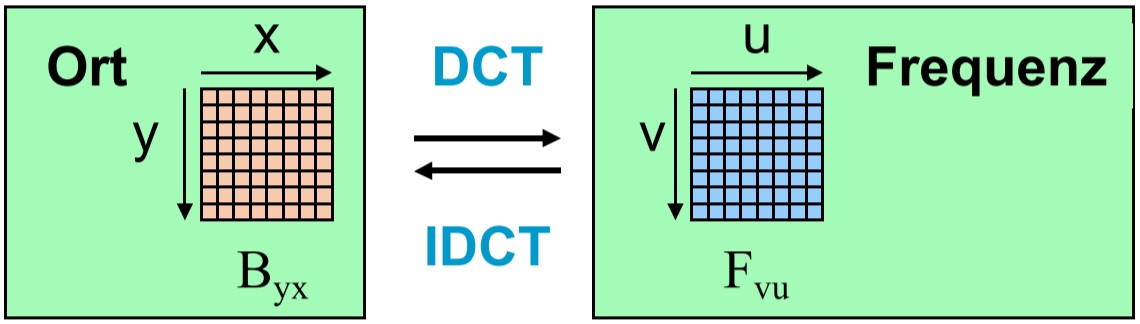
\includegraphics[scale=0.3]{DCT}
\end{center}

\newpage

\subsection{Luminanz und Chrominanz}\label{subsec:luminanz-und-chrominanz}
\begin{multicols}{2}
    \begin{center}
        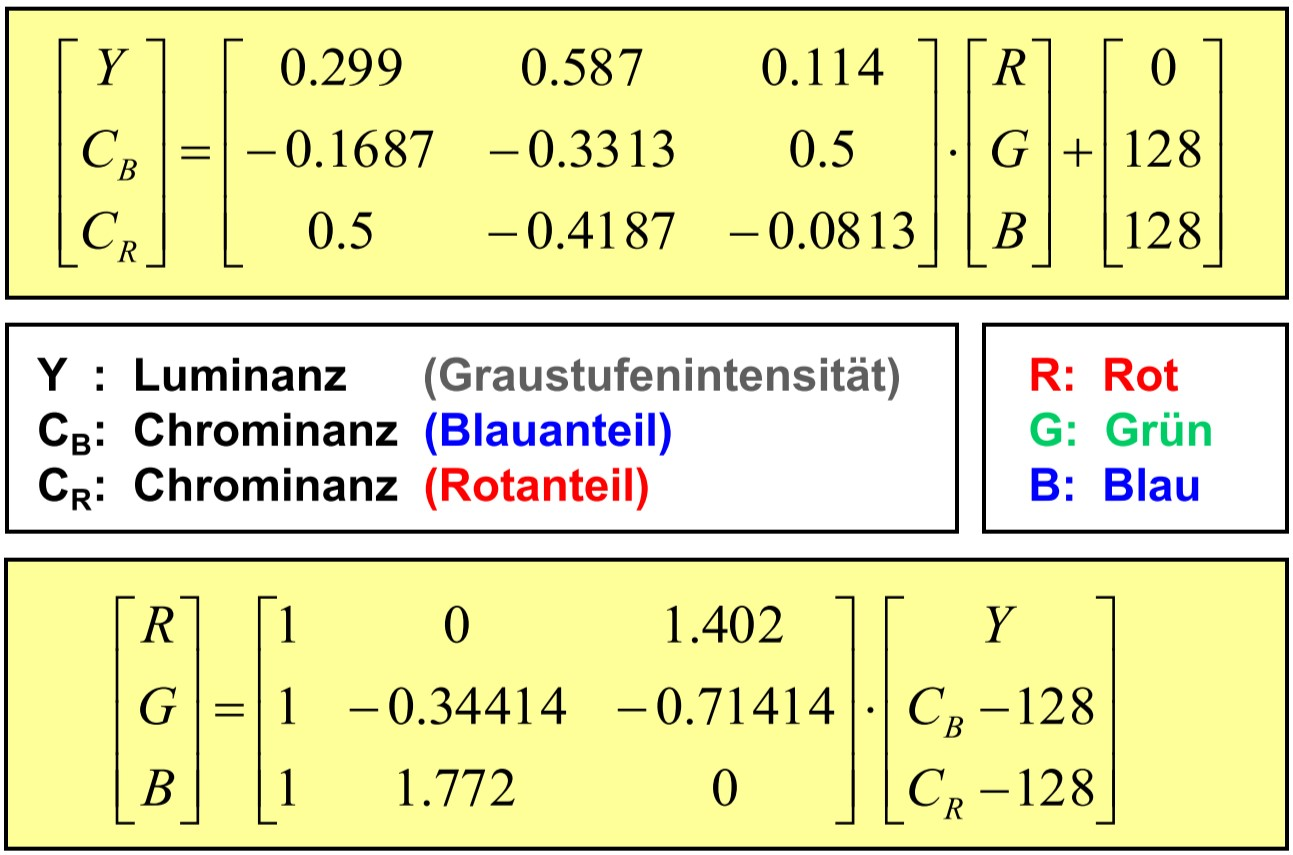
\includegraphics[scale=0.2]{luminanz-chrominanz}
    \end{center}
    \begin{center}
        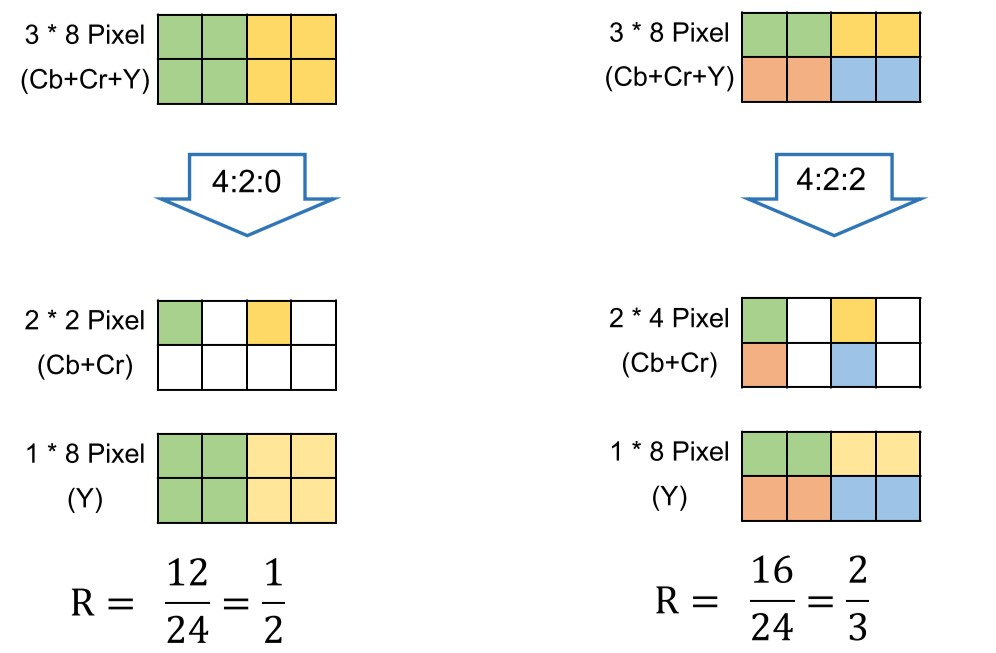
\includegraphics[scale=0.3]{downsampling-example}
    \end{center}
\end{multicols}
\begin{center}
    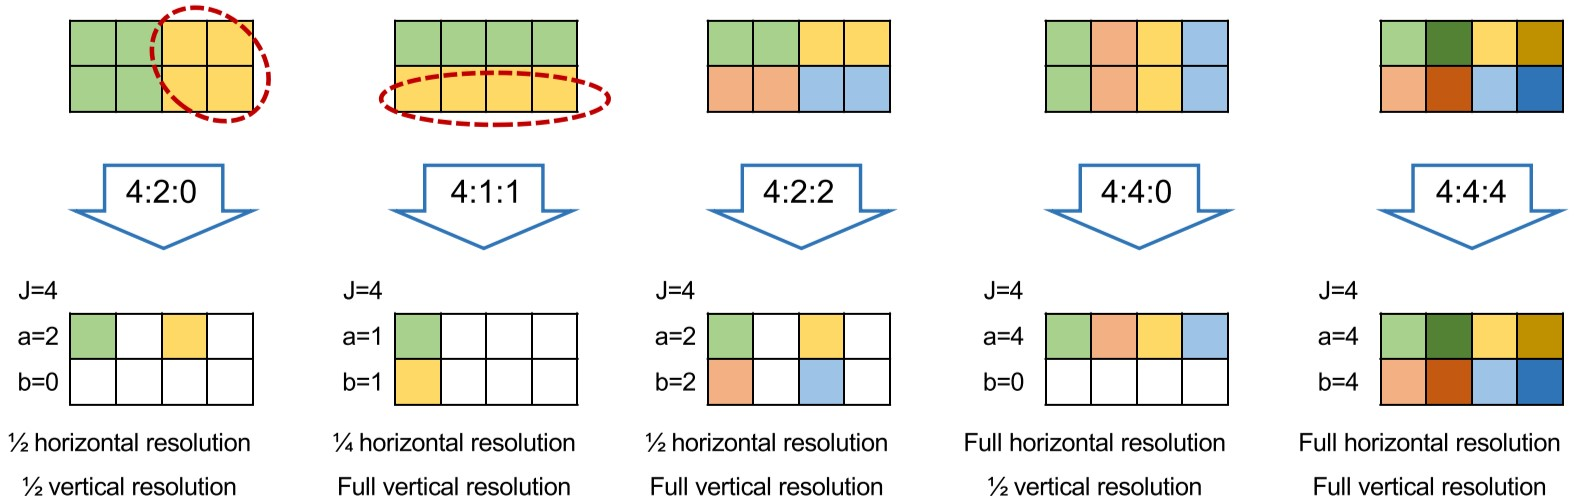
\includegraphics[scale=0.3]{downsampling}
\end{center}

\subsection{JPEG Blockverarbeitung}\label{subsec:jpeg-blockverarbeitung}

\begin{center}
    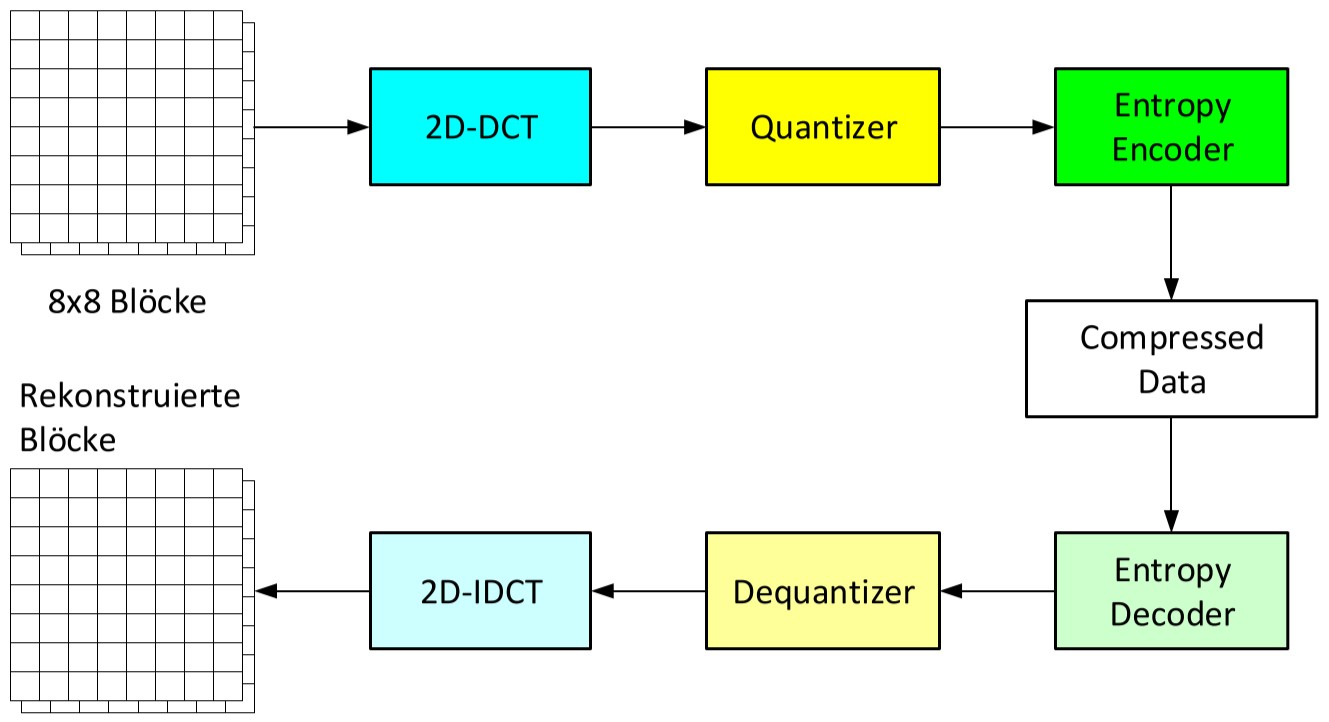
\includegraphics[scale=0.25]{jpeg-blockverarbeitung}
\end{center}

Alle Blöcke zu 8x8 Pixel werden wie folgt weiterverarbeitet:

\begin{itemize}
    \item \emph{Zweidimensionale Diskrete Cosinus-Transformation}: Hierbei werden die Informationen, die als Funktion des Orts vorliegen, in Amplituden von Ortsfrequenzen gewandelt.
    \item \emph{Quantisierer}: Hier wird eine Quantisierung vorgenommen.
    Diese trägt, zusammen mit der Cosinustransformation, wesentlich zur Datenkompression bei, weil bei sehr vielen der insgesamt 64 Werten der Frequenzen nach der Quantisierung der Wert Null übrigbleibt.
    \item \emph{Entropy Encoder}: Die übrigbleibenden relevanten Werten werden nun noch mit einem Entropieverfahren codiert.
    Dies steuert nochmals einen kleinen Beitrag zur gesamten Datenkompression bei.
    Dieser Teil der Kompression ist gänzlich verlustlos, weil Entropieverfahren verlustlos sind.
    \item \emph{Compressed Data}: Die im JPEG-Format komprimierten Daten.
\end{itemize}